%%%%%%%%%%%%%%%%%%%%%%%%%%%%%%%%%%%%%%%%%
% Conference Booklet
% LaTeX Template
% Version 1.0 (22/12/2019)
%
% This template originates from:
% https://www.LaTeXTemplates.com
%
% Authors:
% Maxime Lucas (ml.maximelucas@gmail.com) 
% Pau Clusella
% Modifications for LaTeX Templates by Vel (vel@LaTeXTemplates.com)
%
% License:
% GNU General Public License v3.0
%
%%%%%%%%%%%%%%%%%%%%%%%%%%%%%%%%%%%%%%%%%

%----------------------------------------------------------------------------------------
%	PACKAGES AND OTHER DOCUMENT CONFIGURATIONS
%----------------------------------------------------------------------------------------

\documentclass[
	openany, % Allow chapters to start on odd and even pages
	parskip=full, % Large space between paragraphs
	12pt, % Default font size
	letterpaper, % Paper size, use letterpaper for US letter size
]{conferencebooklet} % Custom class defining the style and layout of the template

\usepackage{hyperref}
\hypersetup{
    unicode=false,          % non-Latin characters in Acrobat’s bookmarks
    pdftoolbar=true,        % show Acrobat’s toolbar?
    pdfmenubar=true,        % show Acrobat’s menu?
    pdffitwindow=false,     % window fit to page when opened
    pdfstartview={FitH},    % fits the width of the page to the window
    pdftitle={John Chiasson Memorial and Symposium},    % title
    pdfauthor={Aykut C. Satici}, % author
    % pdfsubject={Subject},   % subject of the document
    % pdfcreator={Creator},   % creator of the document
    % pdfproducer={Producer}, % producer of the document
    % pdfkeywords={keyword1, key2, key3}, % list of keywords
    pdfnewwindow=true,      % links in new PDF window
    colorlinks=true,       % false: boxed links; true: colored links
    linkcolor=magenta,          % color of internal links (change box color with linkbordercolor)
    linkbordercolor=orange,
    citecolor=blue,        % color of links to bibliography
    citebordercolor=green,
    filecolor=magenta,      % color of file links
    urlcolor=cyan,           % color of external links
    urlbordercolor=blue,
}

%----------------------------------------------------------------------------------------

\begin{document}

%----------------------------------------------------------------------------------------
%	 COVER PAGE
%----------------------------------------------------------------------------------------

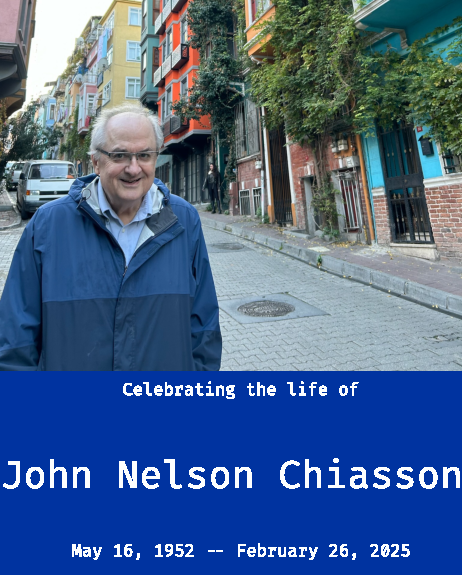
\includepdf{images/cropped_jc.pdf} % The cover for the booklet is included as a whole-page image, it can be a PDF or an image file but must be the same dimensions as the paper size

%----------------------------------------------------------------------------------------
%	 TIMETABLE
%----------------------------------------------------------------------------------------

\chapter{Timetable}

% CT: Contributed Talk, IS: Invited Speaker, KL: Keynote Lecture, IT: Invited Talk.

% \section{Tuesday, 20 of March}
\small{

\begin{longtable}{|C{0.15\linewidth}|  C{0.00\linewidth} C{0.3\linewidth} C{0.0\linewidth} C{0.4\linewidth}|}\hline	
	\tablebreak{10:30 a.m. -- 11:30 a.m.}{Memorial}
	\CT{10:30--10:38}{Amy Fleischer}{Dean of COEN, Boise State}{Introductory remarks}	
	\CT{10:38--10:45}{Neal Bangenter}{Chair of ECE, Boise State}{Chair's perspective of John Chiasson}	
	\CT{10:45 -- 11:00}{Bill Chiasson}{John's twin brother}{Perspectives from John's family}
	\CT{11:00 -- 11:15}{Ruthvik Vaila}{Last PhD student, L. Weston}{Remembering Dr. John Chiasson}
	\CT{11:15 -- 11:30}{Aykut Sat{\i}c{\i}}{Friend/Colleague, Boise State}{John Chiasson: An American Treasure}
	\tablebreak{11:30 a.m. -- 12:15 p.m.}{Refreshments}
	\tablebreak{12:15 p.m. -- 2:30 p.m.}{Symposium}
	\CT{12:15--12:28}{Doug Birdwell}{Univ. of Tennessee, Knoxville}{A Brief Tribute to John Chiasson}
	\CT{12:28--12:41}{Hairong Qi}{Univ. of Tennessee, Knoxville}{Found John! He's at Barnes \& Noble!}
	\CT{12:41 -- 12:54}{Leon Tolbert}{Univ. of Tennessee, Knoxville}{Spacetime PQ Theory for AC and DC Systems}
	\CT{12:54 -- 1:07}{Bob Novotnak}{First PhD student, Aerotech}{Johnny and Bobby - The Early Years}
	\CT{1:07--1:20}{\.{I}nan\c{c} \c{S}enocak}{University of Pittsburgh}{Solving forward and inverse PDE problems with Physics and Equality Constrained Artificial Neural Networks}
	\CT{1:20--1:33}{Burak \"{O}zpineci}{Oak Ridge National Lab.}{Harmonic Optimization and Heat Exchanger Design using Genetic Algorithms}
	\CT{1:33--1:46}{Uri Rogers}{Eastern Washington University}{Differentially Flat Systems and Happiness}
	\CT{1:46-1:59}{Vishal Saxena}{University of Delaware}{Vishal and John's history}
	\CT{1:59-2:12}{Itamar Arel}{Morado Ventures}{John's sabbatical at Itamar's company}
	\CT{2:12-2:25}{Zachary Adams}{Pitch Aeronautics}{Zach and John's collaborations}
	\CT{2:25-2:30}{Remarks from those}{who could not attend}{Hitay \"{O}zbay, Mark W. Spong, Pramod Khargonekar}
\end{longtable}
}

%----------------------------------------------------------------------------------------
%	 USEFUL INFORMATION
%----------------------------------------------------------------------------------------

\chapter{Useful Information}

The memorial and the symposium will be held at the \textbf{Stueckle Sky Center
Loft}, located at 1200 W University Drive, Boise, ID 83706. A map of the
surrounding area is shown in the next page. There will be signage to guide you 
to the particular room where the memorial will be held.

\textbf{Basic refreshments} will be offered after the memorial, leading into the
symposium.

You can park for free in the West Stadium parking lot.

For attending remotely, please use this 
\href{https://www.google.com/url?q=https://boisestate.zoom.us/j/92041896142?pwd%3Dkex70eLC6tKIcjuQ7cW3qPArYgCAMU.1%26jst%3D2&sa=D&source=calendar&ust=1746902820965215&usg=AOvVaw011wx_ahCLtKy9bmFTbUvG}{Zoom link}.

\newpage

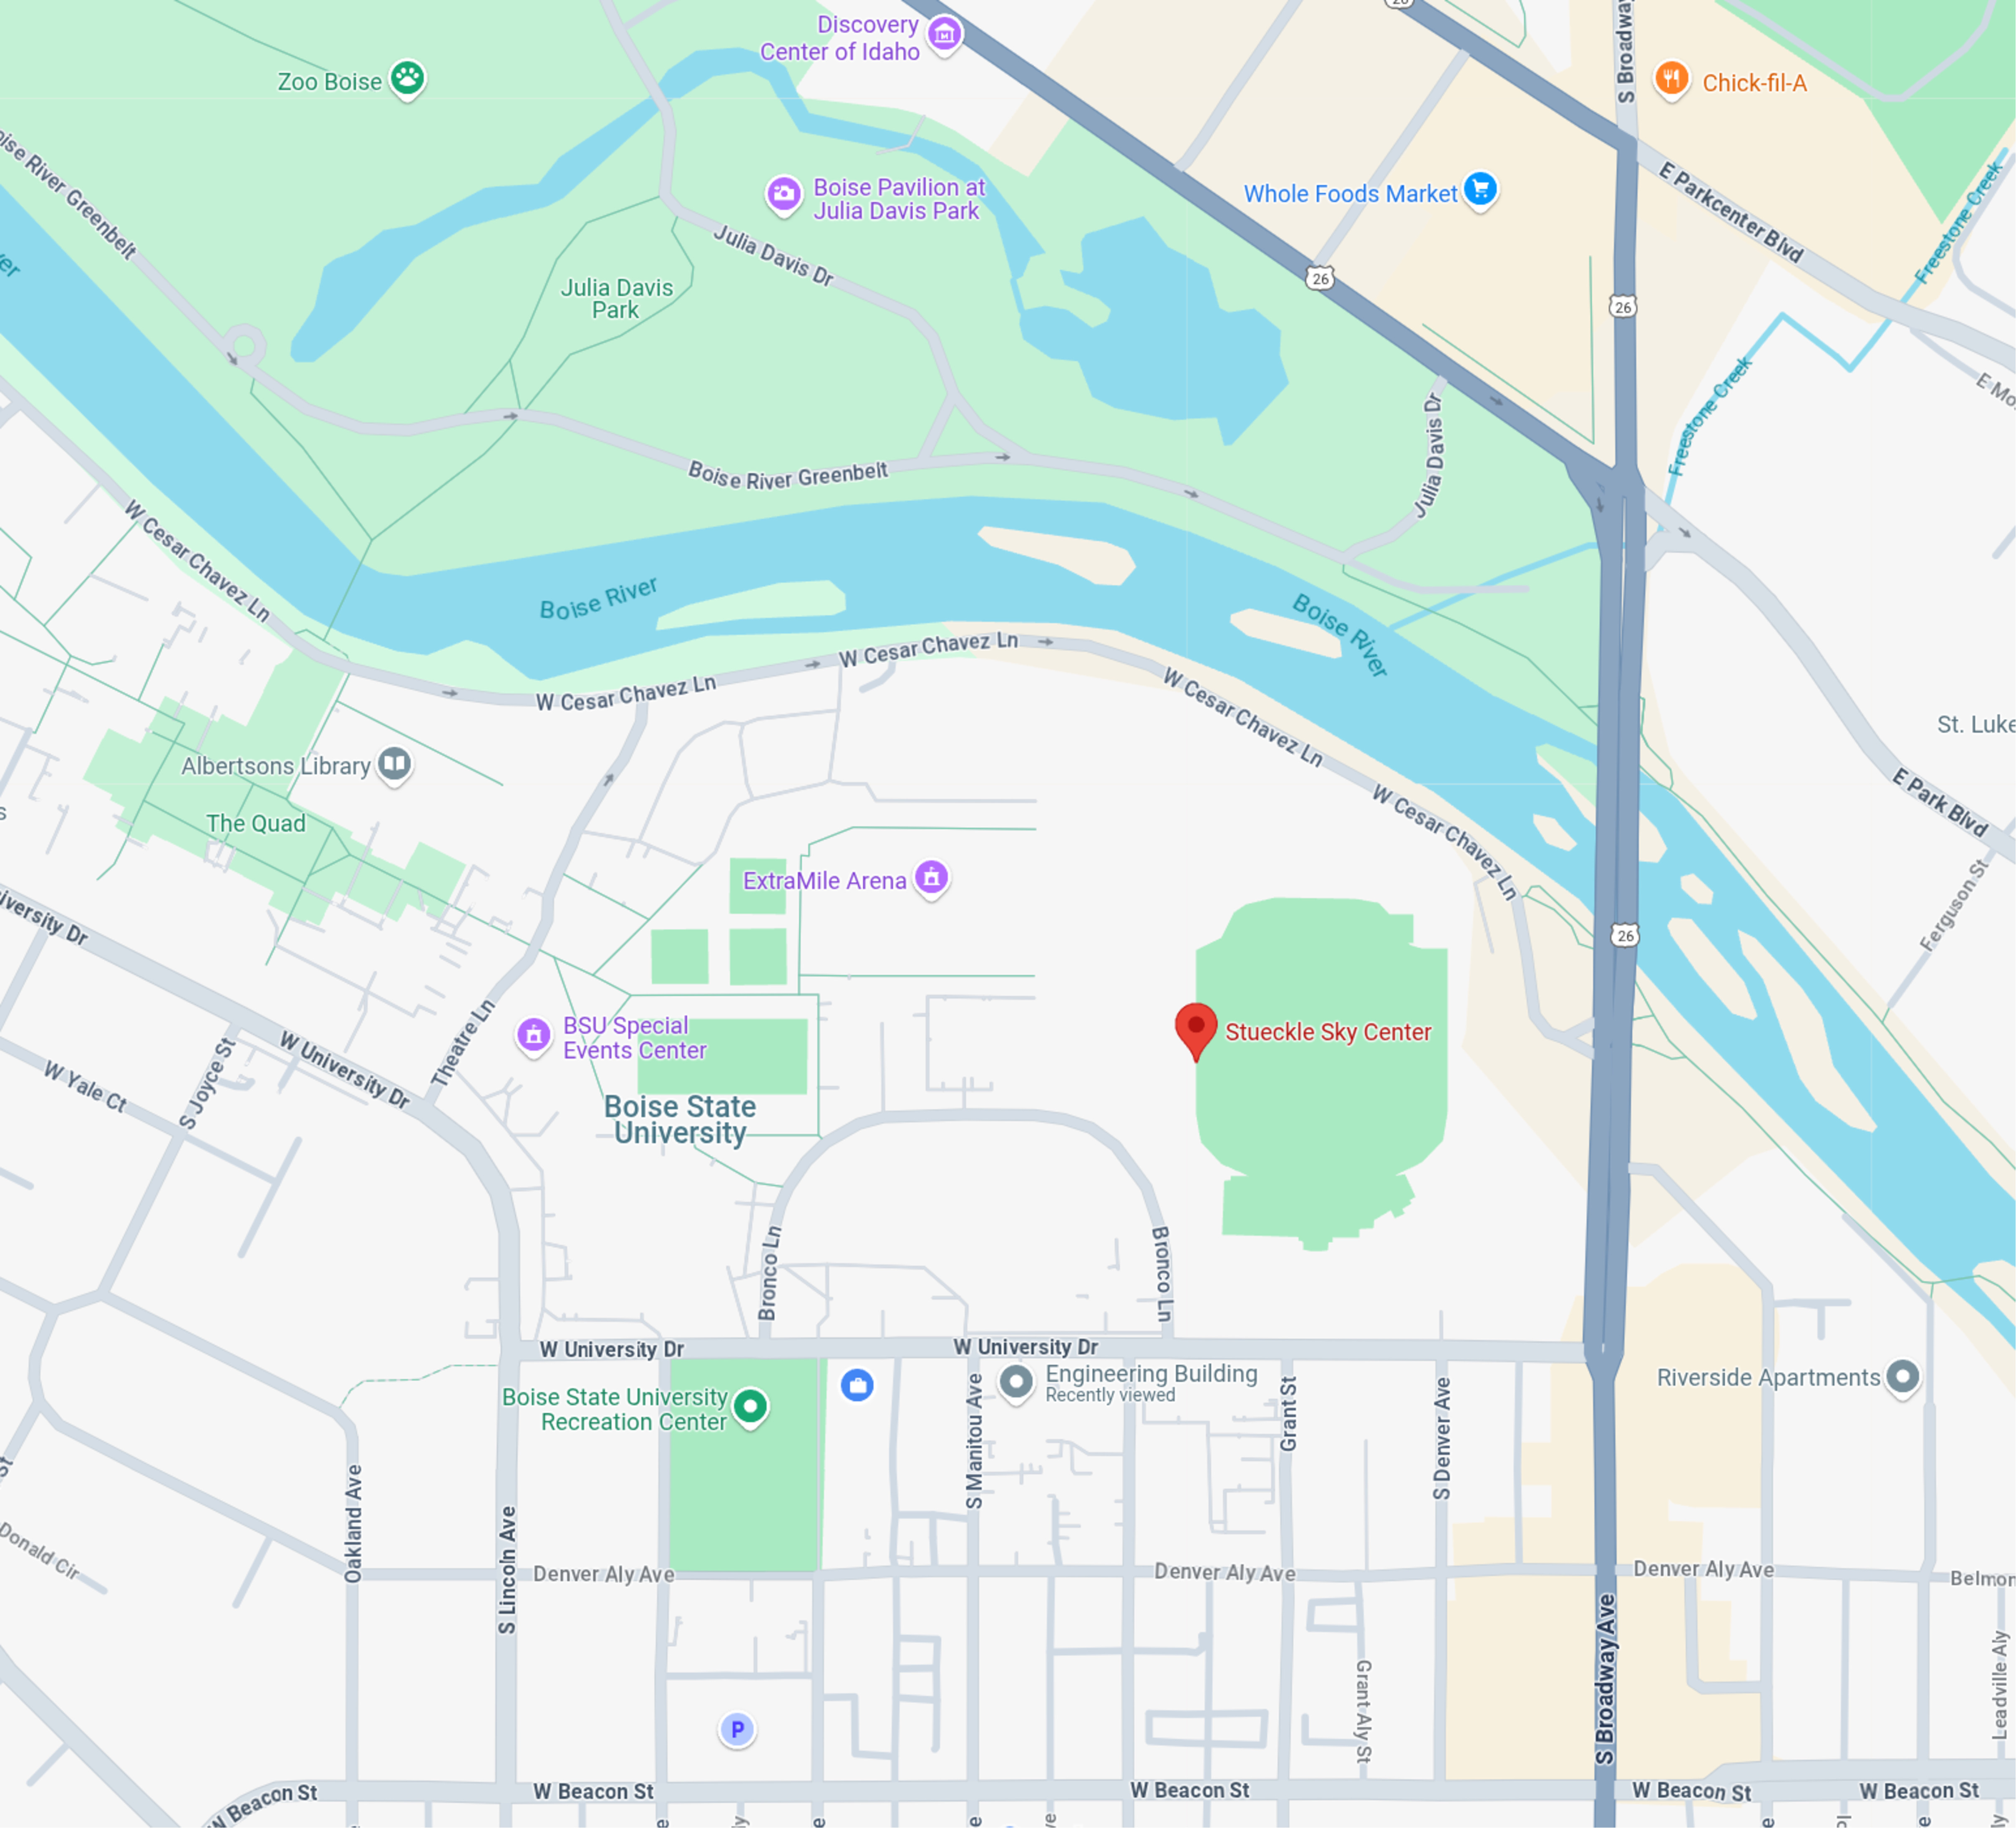
\includegraphics[width=\linewidth]{images/stueckle_map}



%----------------------------------------------------------------------------------------
%	 CLOSING PAGE
%----------------------------------------------------------------------------------------

% \newpage

% \thispagestyle{empty} % Suppress headers and footers on this page
% \pagecolor{myblue} % Coloured background
~

%----------------------------------------------------------------------------------------

\end{document}
